\documentclass[a4paper,10pt]{article}
\usepackage[utf8]{inputenc}
\usepackage{amsmath}
\usepackage{tabularx}
\usepackage{graphicx}
\usepackage{epstopdf}
\usepackage{textcomp}
\usepackage{amsmath}
\usepackage{float}
\usepackage{listings}             % Include the listings-package

\newcolumntype{b}{X}
\newcolumntype{s}{>{\hsize=.25\hsize}X}

%opening
\title{Informe técnico: \\
Adquisición de señales analógicas}
\author{P. Domenichini, A. Mendez}

\begin{document}

\maketitle

% Objetivos de mínima
% 1. Buscar y elegir una librería para control de la placa de audio.
% 2. Caracterizar la entrada de la placa de audio.
% 3. Caracterizar la salida de la placa de audio.
% 4. Reemplazar en el programa del día anterior el generador de
%    funciones o el osciloscopio por la placa de audio.
% 5. Curva de respuesta: Diodo, BJT o JFET
% 6. Implementar un circuito aplicando OPAMP o Regulador LM317
% 7. Armar una hoja de datos para reportar resultados

% Lineamientos
% I Formato tipo informe técnico
% I Detalles más relevantes del programa (diagrama de flujo, pseudocódigo, etc)
% I Descripción experimental
% I Especificar el programa utilizado para cada medición (si corresponde...)
% I Resumen de resultados tipo “hoja de datos”

\section{Placa de audio}
La adquisición de señales analógicas mediante control de placa 
de audio del presente trabajo se realizo a través de la utilización
de la librería {\sc pyaudio}. 


\subsection{Emisión y adquisición de señal con python}
La emisión y adquisición de señales mediante el uso de la placa
de audio se realizo con dos programas independientes de lectura y escritura. 
Por ejemplo, el código de lectura que nos permitió
adquirir las señales relevantes de los circuitos implementados en las 
secciones \ref{sec:diodo} y \ref{sec:opamp} tiene una estructura similar 
a la del siguiente código:

\lstset{language=Python}
\begin{lstlisting}[frame=single]  % Start your code-block

import pyaudio
import numpy as np
p = pyaudio.PyAudio()
ftype=pyaudio.paInt16
nbuff=44100
stream = p.open(format=ftype,channels=2,
                rate=nbuff,input=True)
data = stream.read(nbuff)
stream.stop_stream()
stream.close()
p.terminate()
audioin_data = np.fromstring(data, np.int16)
\end{lstlisting}
% 
% \lstset{language=Python}
% \begin{lstlisting}[frame=single]  % Start your code-block
% 
% import pyaudio
% import numpy as np
% def sine(freq):
%    xfreq=int(nbuff/freq)
%    ntimes=int(duration*xfreq)
%    x=np.arange(xfreq*ntimes)
%    out=amp*np.sin(2*np.pi*x/xfreq)
%    return out.astype(np.float32)
% ftype=pyaudio.paFloat32
% nbuff=44100       # float32 sampling rate, Hz (int)
% duration=10.0      # in seconds
% amp=2**8/2        # wave amplitude
% volume=1.0        # range [0.0, 1.0] * amp
% freq=10000.0       # sine frequency, Hz
% samples=sine(freq)
% p = pyaudio.PyAudio()
% stream=p.open(format=ftype,channels=1,
%               rate=nbuff,output=True)
% stream.write(volume*samples)
% stream.stop_stream()
% stream.close()
% p.terminate()
% \end{lstlisting}

\subsection{Respuesta en frecuencia de la placa de audio}

En el modo de emisión de señales, para reportar los valores máximos 
y mínimos de frecuencia, se realizó un barrido de frecuencias entre 
los valores 1 y 10000 Hz. La respuesta de la placa de sonido fue
buena para valores de frecuencia menores a 10 Hz. Para valores
menores a 10 Hz, se pudo observar que la señal empezaba a deformarse.
Esto se debe a que el sistema actúa como un pasa altos a partir de 
dicho valor. Los resultados obtenidos se muestran en la Figura 
\ref{fig:frecuenciaminima}. En el caso del límite máximo, la
respuesta de la placa alcanzó los 10000 Hz. Para valores mayores, la
señal saturaba, produciendo una señal de salida de dicha frecuencia
máxima. 

\begin{figure}[h!]
 \centering
 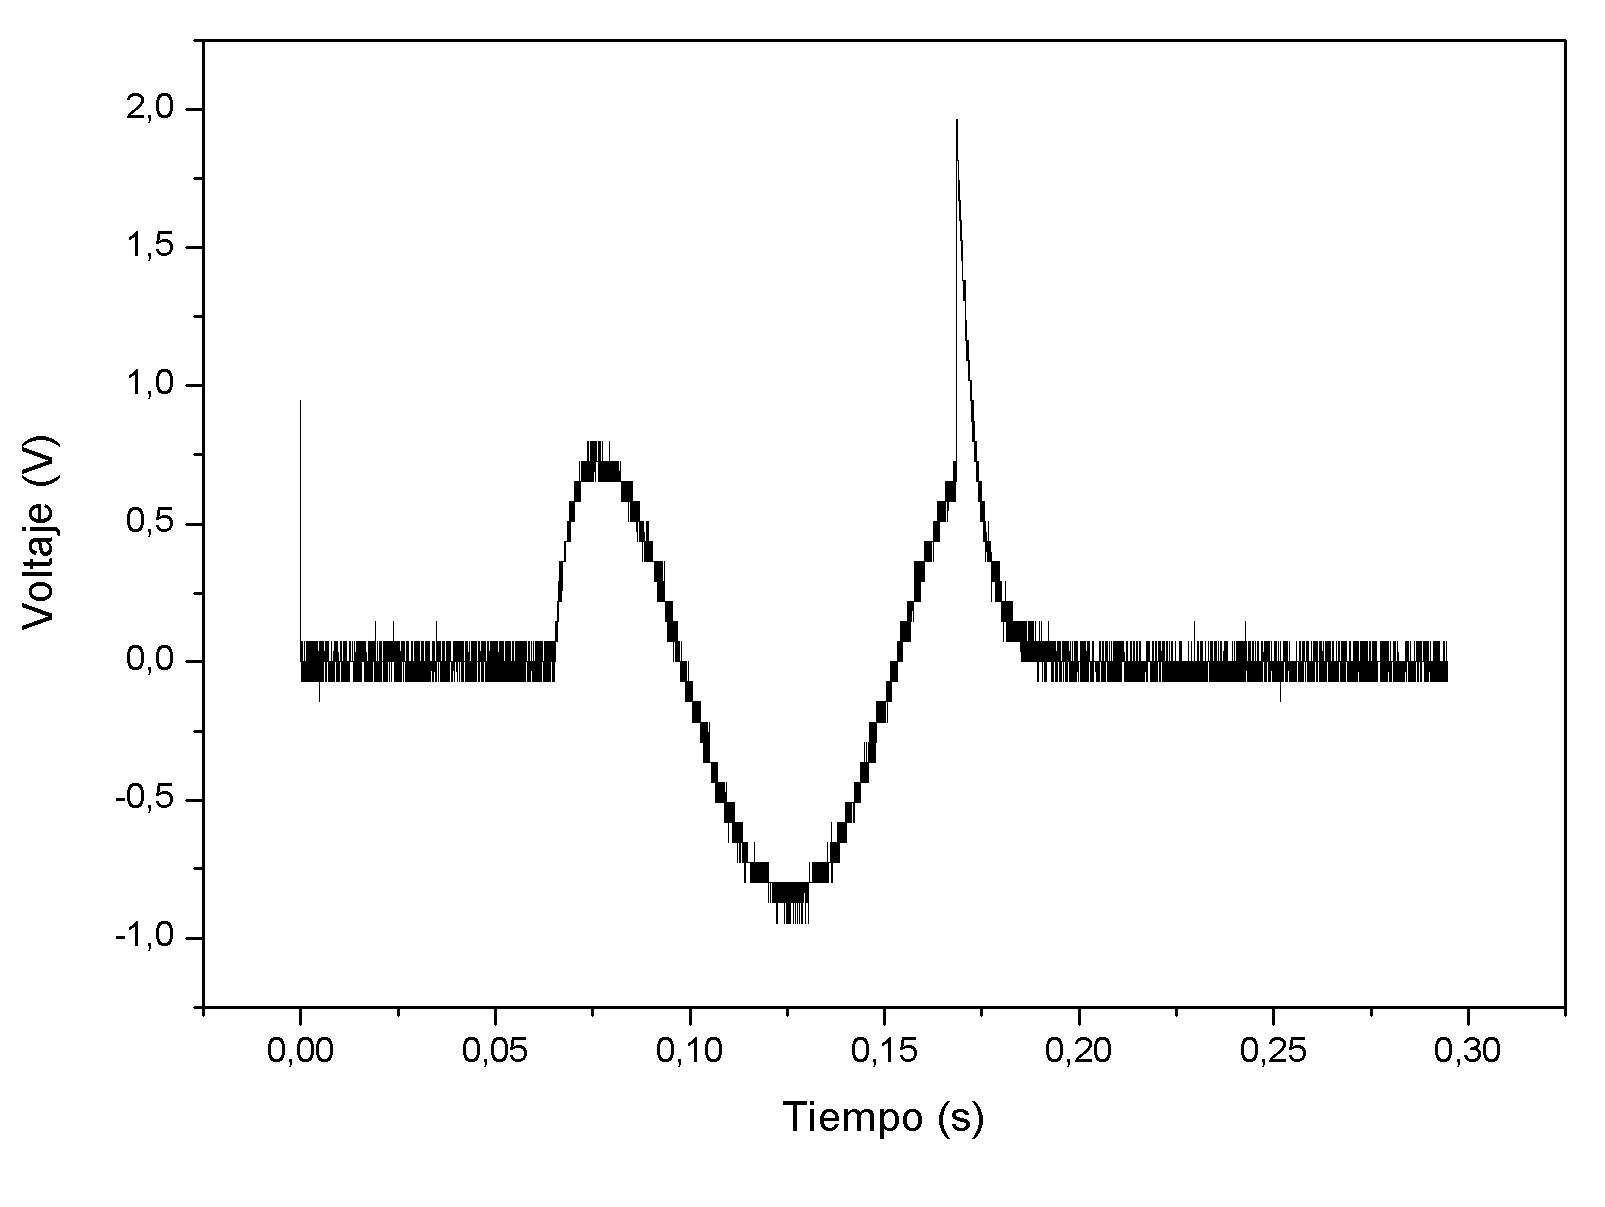
\includegraphics[width=0.40\textwidth]{V2-f1Hz.jpg} (a)
 \hspace{0.1cm}
 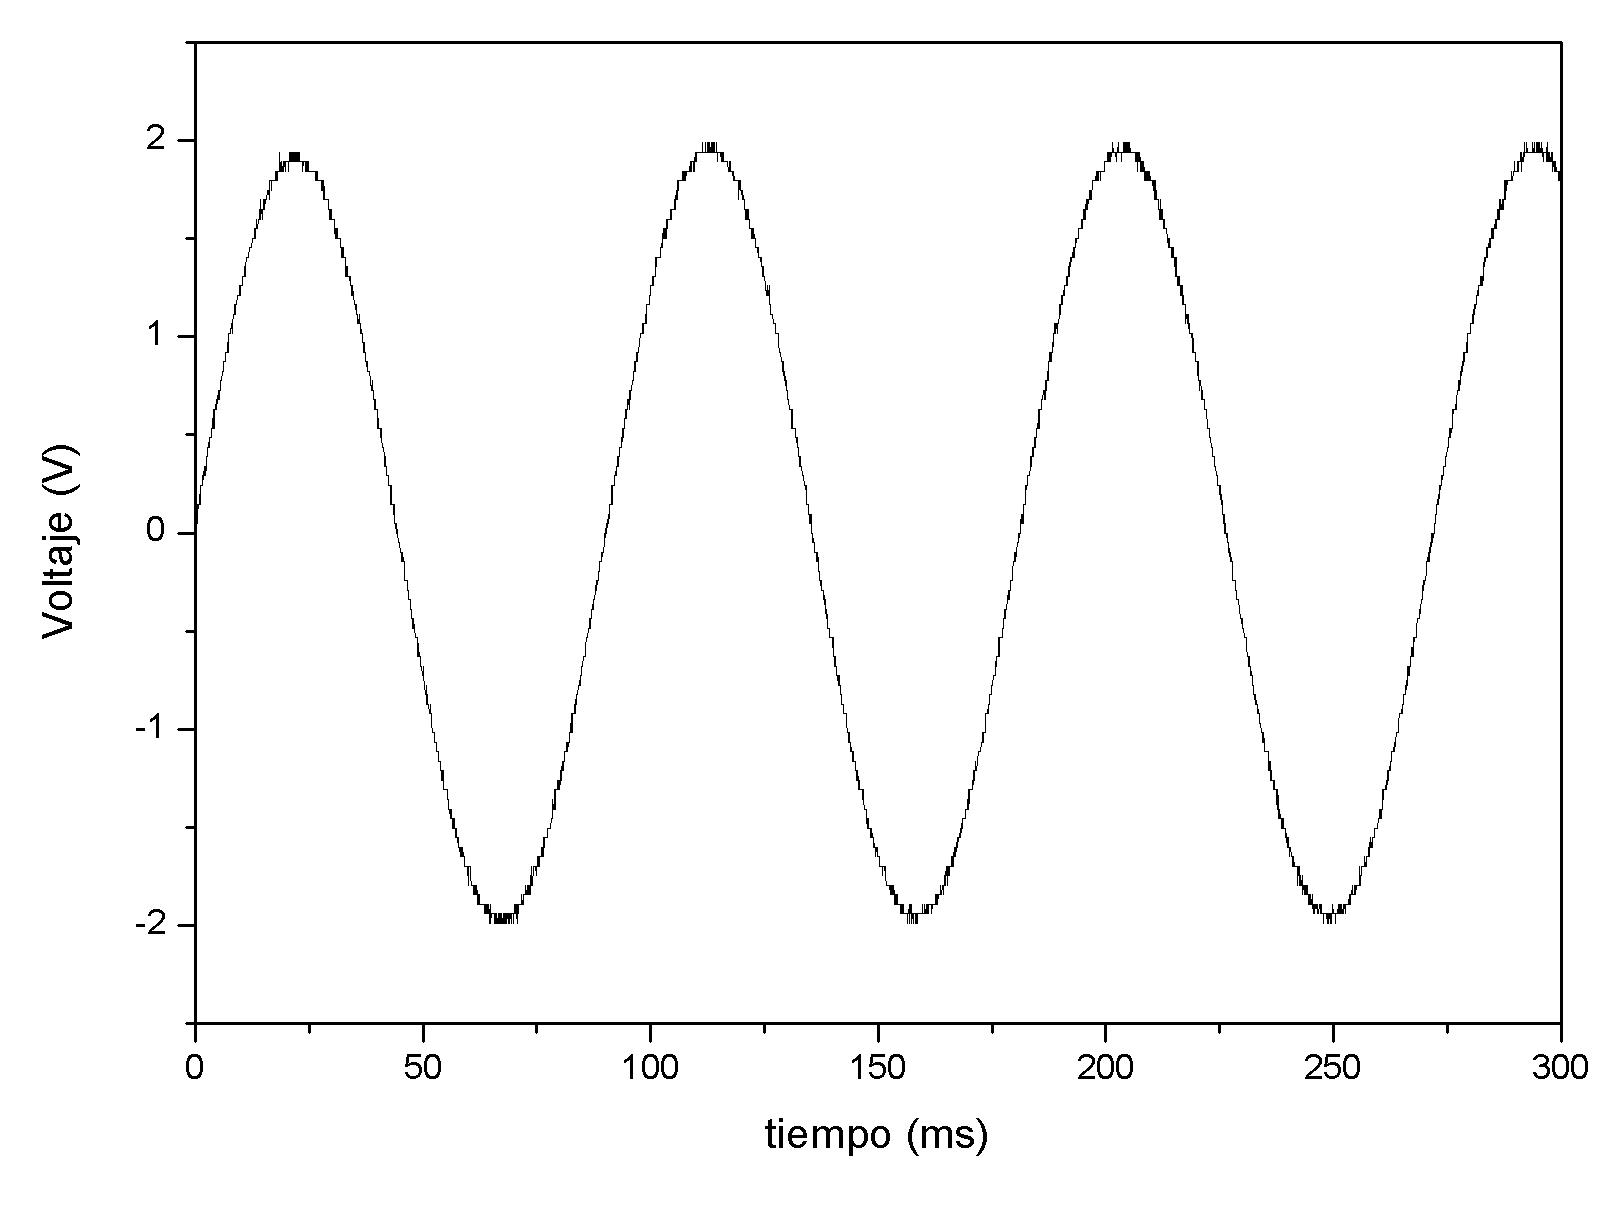
\includegraphics[width=0.40\textwidth]{V2-f10Hz.jpg} (b)
 \label{fig:frecuenciaminima}
 \caption{Medidas de la señal de salida de una onda sinusoidal de la 
 placa de audio para 1 Hz (a) y 10 Hz (b).}
\end{figure}

\subsection{Respuesta en voltaje de la placa de audio}
Para analizar los valores de voltaje que pueden aplicarse con la
placa de audio se utilizaron variables del tipo Float32, con 
valores entre 1 y $-1$. A partir de valores mayores a 
$\pm1$, la señal saturaba, lo que resultaba en una deformación de 
la señal de salida. 

\begin{figure}[h!]
 \centering
 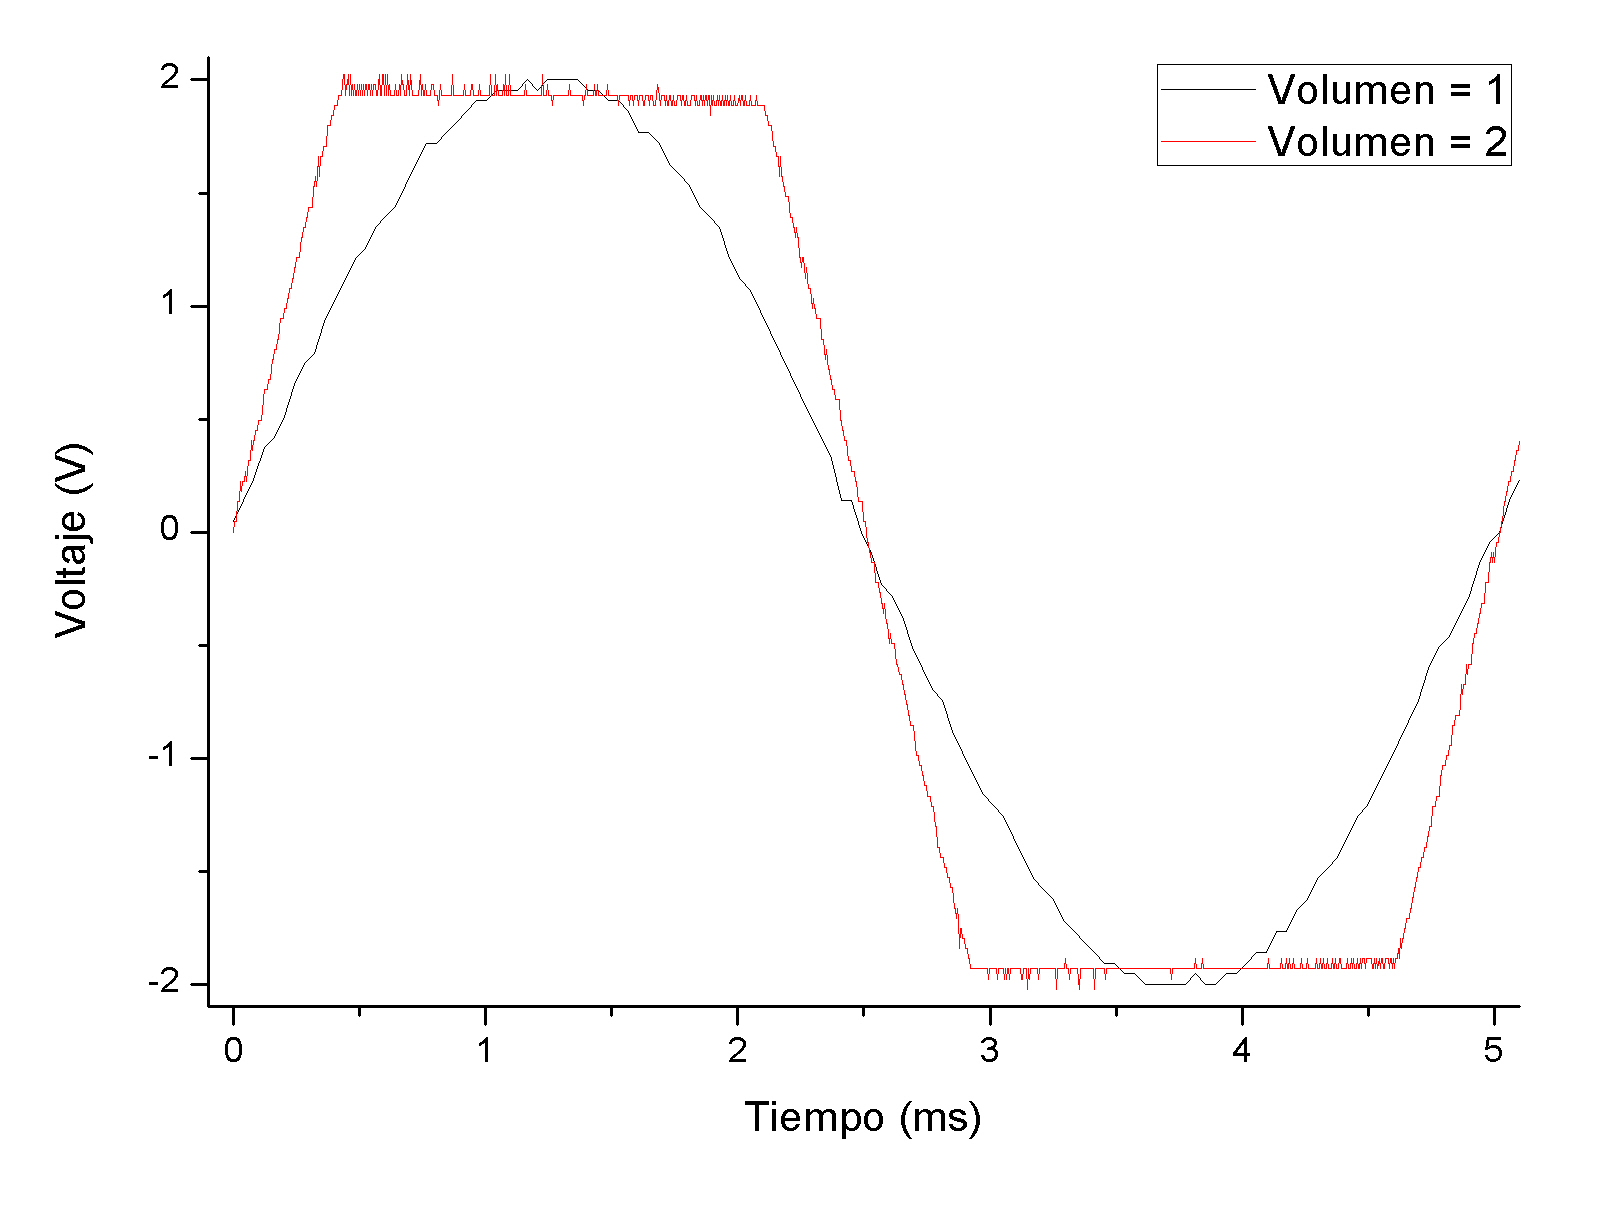
\includegraphics[width=0.40\textwidth]{Entrada-Volumen.jpg} (a)
 \hspace{0.1cm}
 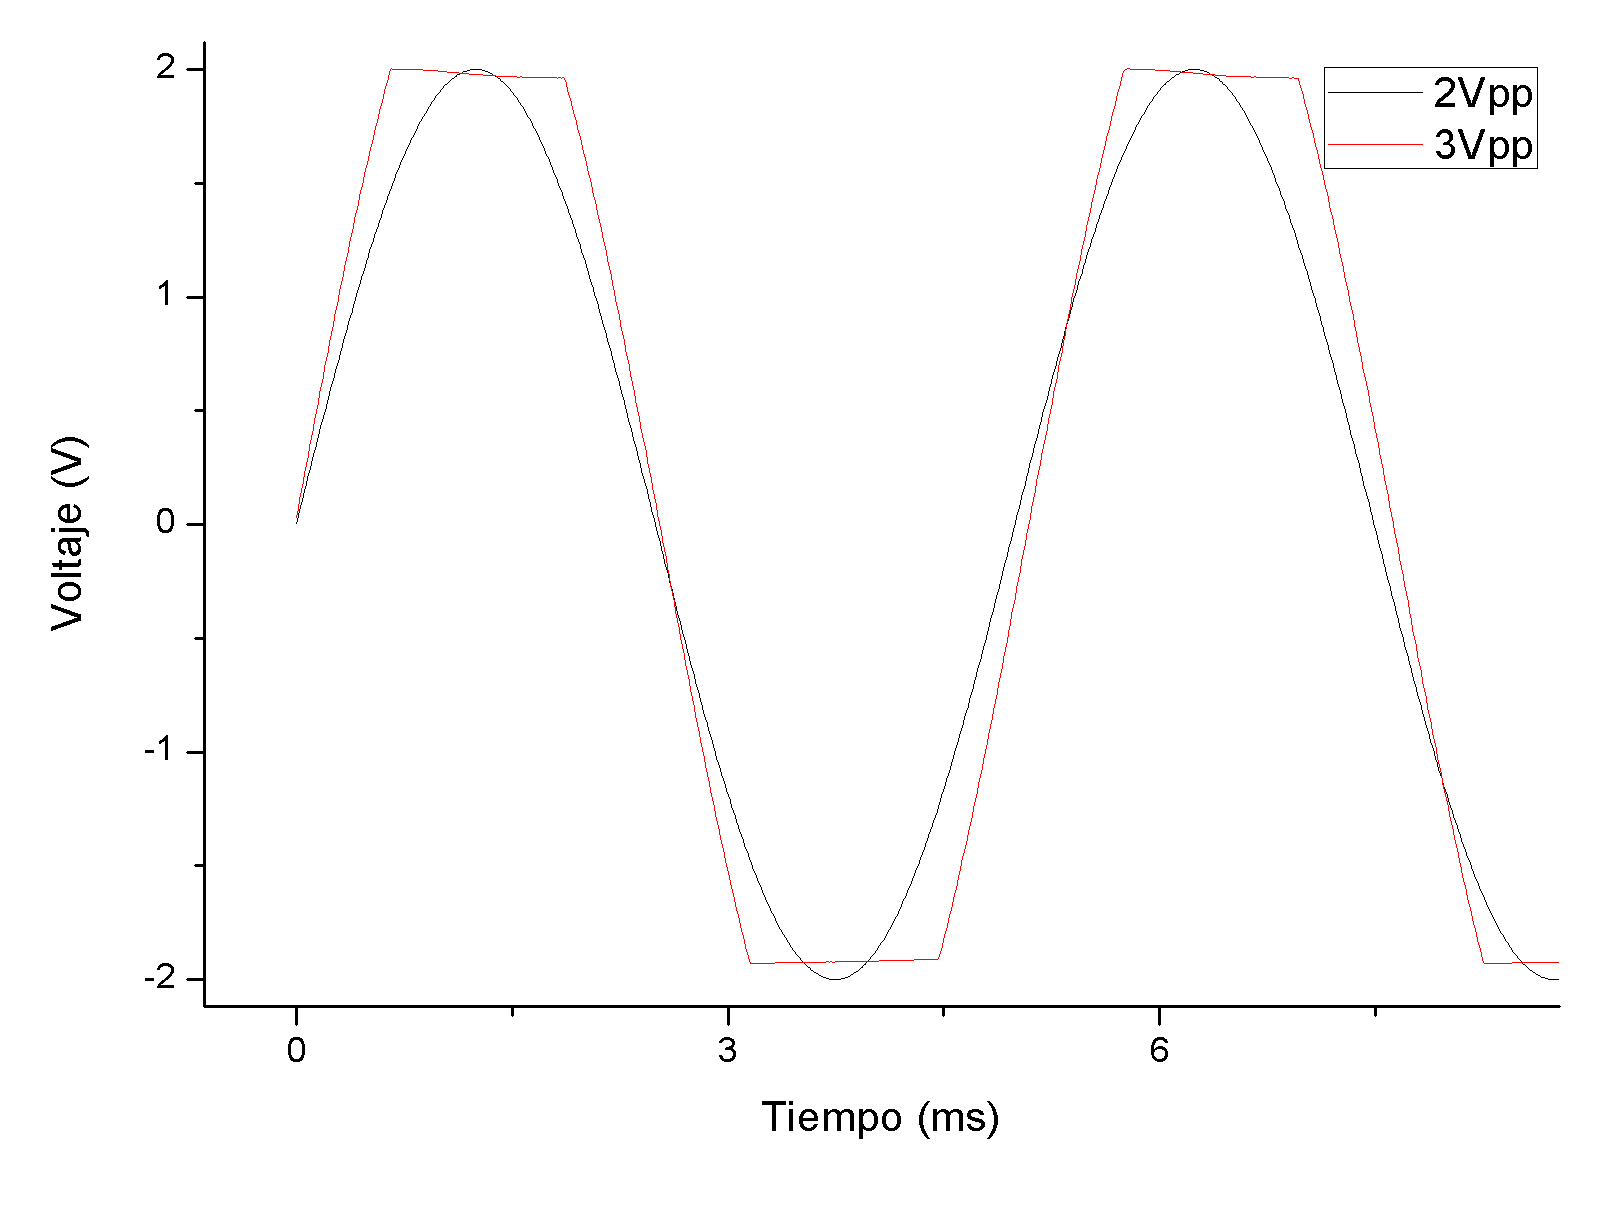
\includegraphics[width=0.40\textwidth]{PlacaAudio-Adq.jpg} (b)
 \label{fig:frecuenciaminima}
 \caption{Medidas de la señal de salida de la placa de Audio para ondas 
 sinusoidales con frecuencia de 200 Hz y con el volumen máximo $V=1$ (a) 
 e intentando sobrepasarlo $V=2$ (b).}
\end{figure}

Un resumen de la caracterización de entrada y salida de la placa de
audio utilizada puede encontrarse en la Tabla~\ref{tab:inout-audio}.
\begin{table}[h]
\begin{tabularx}{\textwidth}{b|s|s|s }
Característica & Min & Máx & Unidad \\
\hline
Voltaje señal de entrada & 2 & -2 & V \\ 
Voltaje señal de salida & -2 & 2 & V \\
Frecuencia señal de entrada & 1 & 10000 & Hz \\
Frecuencia señal de salida & 10 & 10000 & Hz 
\end{tabularx}
\label{tab:inout-audio}
\caption{Caracterización de señales de entrada y salida de la placa 
de audio.}
\end{table}


\section{Determinación de curva de respuesta de diodo}
\label{sec:diodo}

Para probar las capacidades básicas de la placa de audio como
generador de ondas, se medió la curva de voltaje--corriente de
un diodo. Para esto, se implementó el circuito que se muestra en la 
Figura~\ref{fig:diodo}a. La curva I-V de respuesta del diodo se
muestra en la Figura~\ref{fig:diodo}b. Para poder definir las 
tierras del circuito de manera correcta, las conexiones de la señal
de salida recolectadas por el osciloscopio fueron definidas de forma
invertida. De manera, que la señal recolectada fue posteriormente
multiplicada por $-1$.
%Cabe destacar que a la curva obtenida se multiplicaron por -1, dado que por la forma en que se conectó el osciloscopio, para que no haya problemas de tierras, estos valores estaban invertidos. 
La señal de entrada generada por la placa de audio tenía 2~V de 
amplitud y una frecuencia de 200~Hz.
\begin{figure}[h!]
 \centering
 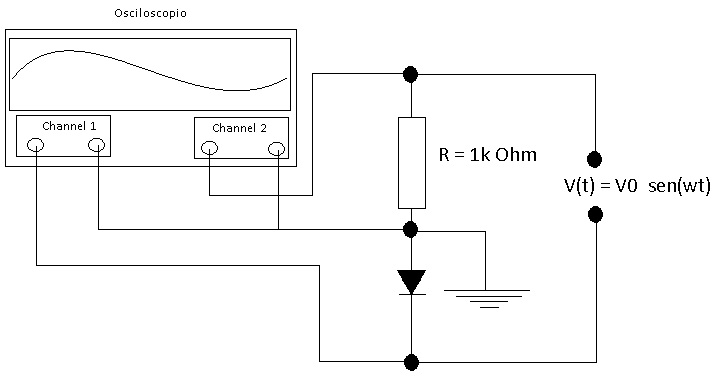
\includegraphics[width=0.5\textwidth]{circuit.jpg} (a)
 \hspace{0.1cm}
 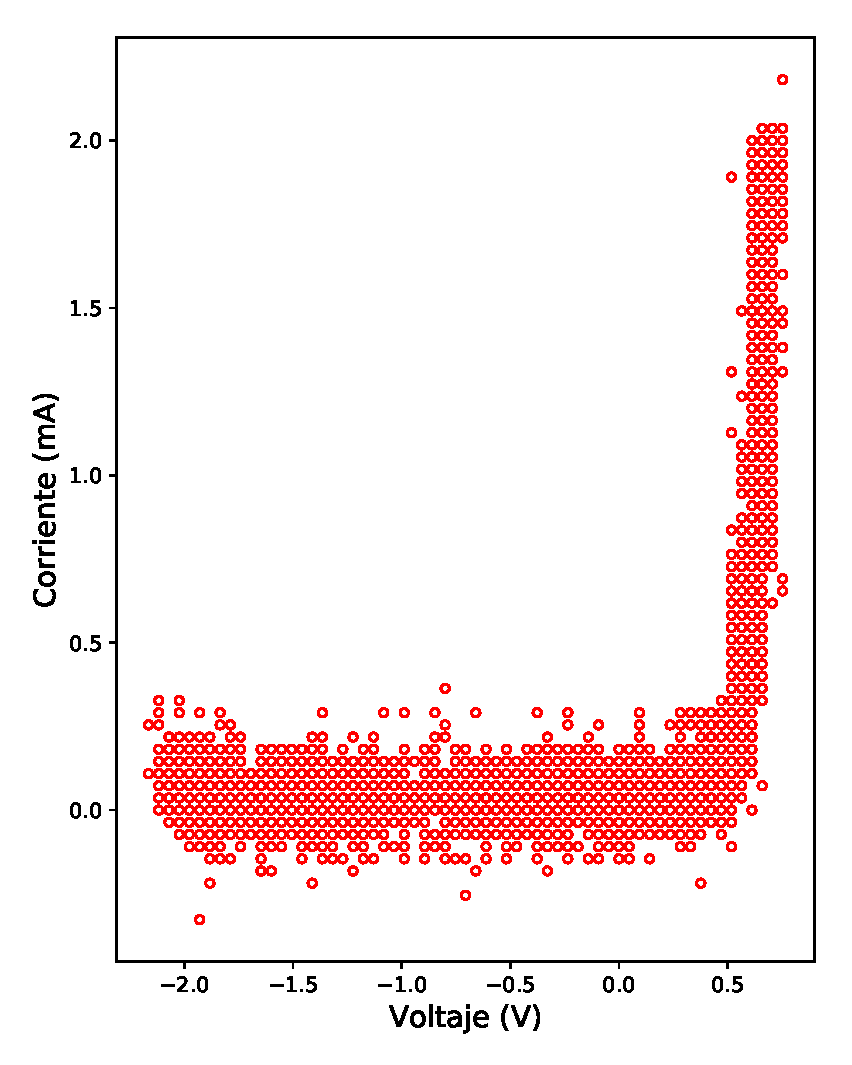
\includegraphics[width=0.35\textwidth]{diodo.eps} (b)
 \label{fig:diodo}
 \caption{(a) Esquema del circuito implementado. 
 (b) Curva I-V del diodo.}
\end{figure}


\section{Implementación de OPAMP}
\label{sec:opamp}

Se puso en práctica el diseño de un circuito con amplificador 
operacional que permita determinar el {\it slew rate} de un
OPAMP. El diagrama del circuito implementado con tal fin se 
muestra en la Figura~\ref{fig:opamp}, en el que se implementó
un LM741.
\begin{figure}[h]
 \centering
% 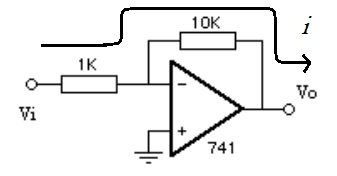
\includegraphics[width=0.4\textwidth]{AmpInv.png}(a)
% \hspace{0.1cm}
 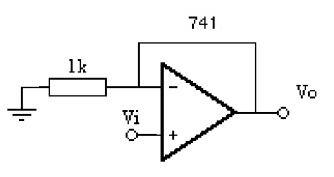
\includegraphics[width=0.4\textwidth]{slewratecircuit.png}
 \label{fig:opamp}
 \caption{Diseño del circuito para determinar el slew rate.}
\end{figure}
Para la medición del slew rate, se definieron dos señales de 
entrada, 2~$V_{PP}$ y 5~$V_{PP}$. La primera se muestra en la
Figura~\ref{fig:slewrate} con puntos rojos. Las frecuencias de 
las señales de entrada en ambos casos fueron iguales a 1kHz. 
Debido a la limitación de voltaje en la señal proveída por la
placa de audio (ver Tabla~\ref{tab:inout-audio}), la señal de 
5~$V_{PP}$ se encontraba saturada. Así, la medición del slew rate
no pudo ser realizada con éxito mediante la utilización de la 
placa de audio. 
\begin{figure}[H]
 \centering
 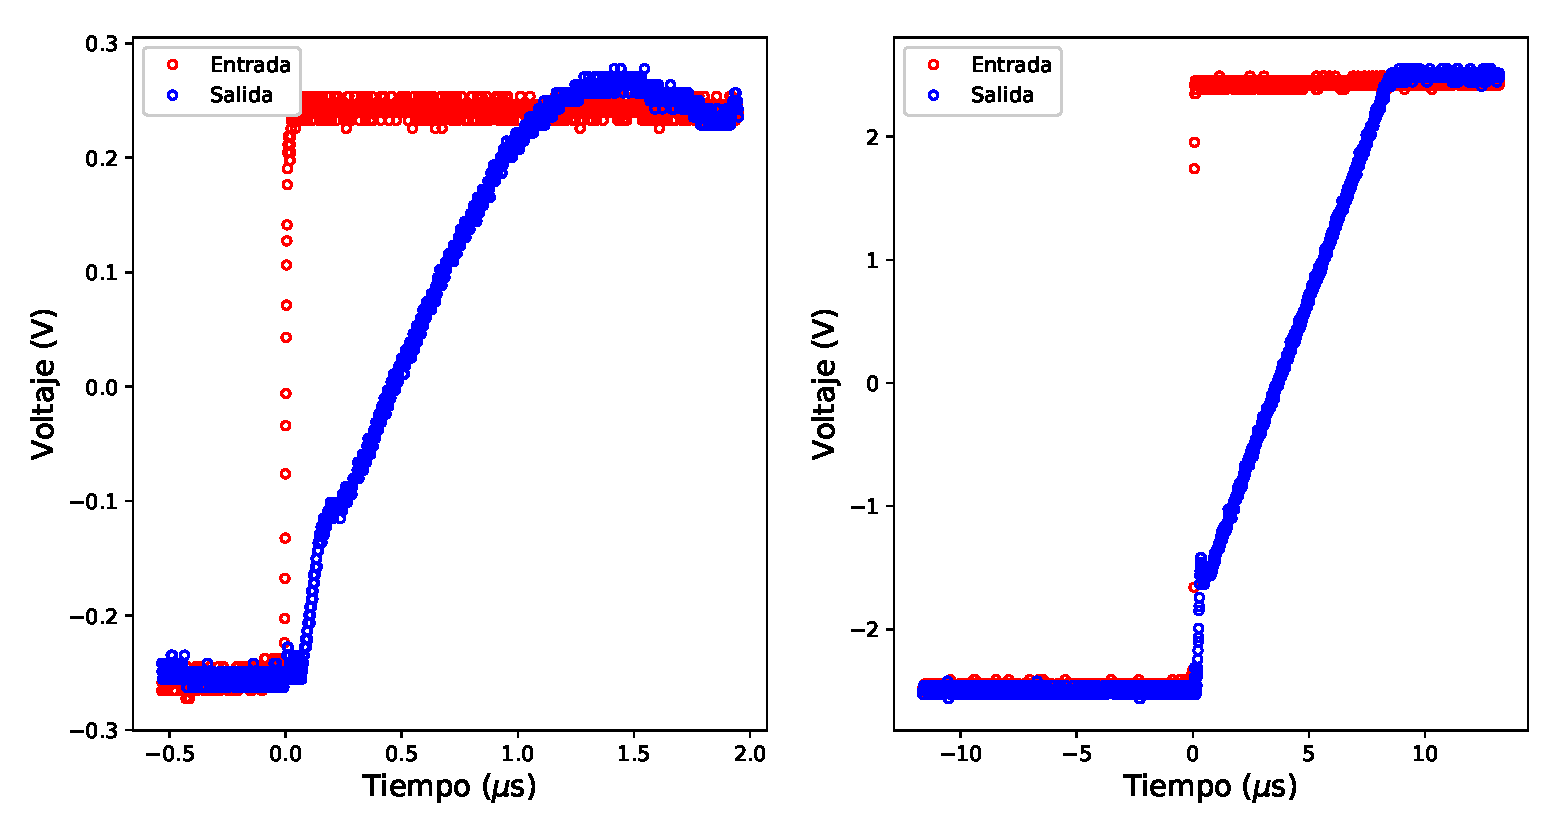
\includegraphics[width=0.7\textwidth]{slewrate.eps} \\
 \hspace{0.2cm}(a)\hspace{4.5cm}(b)
 \label{fig:slewrate}
 \caption{Señales de entrada y salida de una onda cuadrada de
 2 V$_{PP}$ (a) y 5 V$_{PP}$ (b) y 5kHz de frecuencia.}
\end{figure}

\end{document}
